\documentclass[varwidth]{standalone}[2011/222/21]
\usepackage{pgfplots}
\renewcommand*{\familydefault}{\sfdefault}
\pgfplotsset{compat=1.17}
\usepackage{xcolor}

\definecolor{BLUE-light}{rgb}{0.29, 0.59, 0.82}
\definecolor{BLUE-cu}{rgb}{0.7, 0.75, 0.71}
\definecolor{red-cu}{rgb}{0.9, 0.4, 0.38}

\begin{document}
\begin{figure}[htb]
  \begin{minipage}{\textwidth}
    \centering
    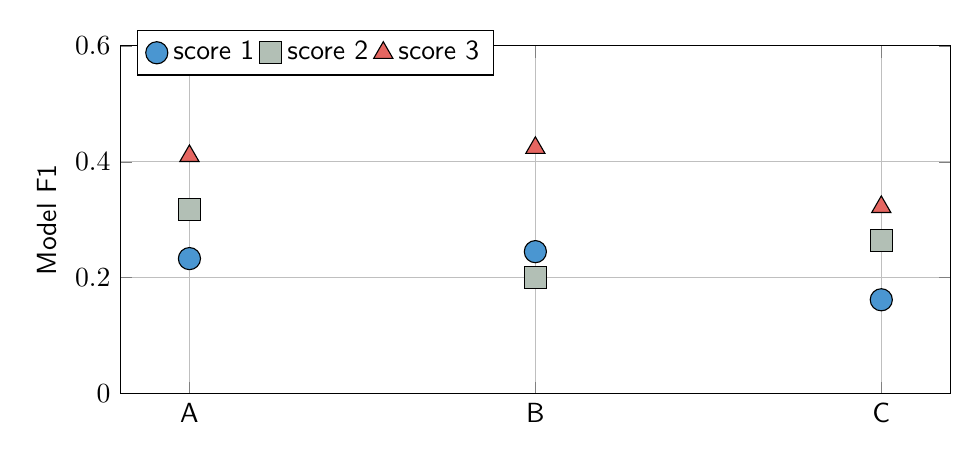
\begin{tikzpicture}
      \begin{axis}[
        /pgf/number format/1000 sep={.},
        width=\textwidth,
        height=6cm,
        symbolic x coords={A, B, C},
        xtick=data,
        ymin=0,ymax=0.6,
        ylabel={Model F1},
        legend pos=north west,
        legend style={at={(0.02,0.98)},anchor=west,legend columns=-1},
        legend entries={score 1, score 2, score 3},
        grid=major,
      ]
      
      \addplot[only marks, mark=*, mark options={fill=BLUE-light,  mark size=4}] coordinates {
        (A, 0.233)
        (B, 0.245)
        (C, 0.162)

      };
      
      \addplot[only marks, mark=square*, mark options={fill=BLUE-cu, mark size=4}] coordinates {
        (A, 0.318)
        (B, 0.200)
        (C, 0.264)

      };

      \addplot[only marks, mark=triangle*, mark options={fill=red-cu,  mark size=4}] coordinates {
        (A, 0.410)
        (B, 0.424)
        (C, 0.322)
      };
      \end{axis}
    \end{tikzpicture}
  \end{minipage}
\end{figure}
\end{document}


